\documentclass{article}

\usepackage{hyperref}
\usepackage{amssymb,amsfonts,amsmath,amsthm}
\usepackage[dvipsnames]{xcolor}
\usepackage{enumerate,enumitem,tikz-cd,tikz,mathrsfs,graphicx,marvosym,wasysym,epigraph,afterpage}
%mathrsfs is for \mathscr, marvosym for \Coffeecup, graphicx for \heartsuit, wasysym is for \twonotes
%\usepackage[colorlinks=true, urlcolor=purple, linkcolor=RoyalBlue, citecolor=magenta, pdfborder={0 0 0}]{hyperref}
%\usepackage[document]{ragged2e}
\usetikzlibrary{backgrounds}

\setlength\epigraphwidth{.6\textwidth}
%\setlength\epigraphrule{0pt}
\setlength{\parindent}{0pt}

\newcommand\blankpage{
    \null
    \thispagestyle{empty}
    \addtocounter{page}{-1}
    \newpage}

\newtheorem{thm}{Theorem}[section]
\newtheorem{cor}[thm]{Corollary}
\newtheorem{prop}[thm]{Proposition}
\newtheorem{lem}[thm]{Lemma}
\newtheorem{defn}[thm]{Definition}
\theoremstyle{definition} 
\newtheorem{exmp}[thm]{Example}
\newtheorem{rem}[thm]{Remark}

\newcommand{\Z}{\mathbb{Z}}
\newcommand{\Oo}{\mathcal{O}}
\newcommand{\ts}{\mathrm{ts}}
\newcommand{\tee}{\mathfrak{t}}



\begin{document}
\begin{titlepage}
\end{titlepage}




\subsection{The (he)art of gluing} The slice functor hides greater potential. Indeed, even if we don't have a morphism of $\mathbb{Z}$-posets (but just a $\mathbb{Z}$-equivariant map), then the slice functor can still be applied, obtaining a partially defined map. \\

Let $J$ be a $\Z$-poset, i.e., a partially ordered set together with a monotone action of $\Z$, that we will denote by $(n,x)\mapsto x+n$. Recall that a $J$-slicing on a stable $\infty$-category $\mathscr{D}$ is a morphism of $\Z$-posests $\tee\colon \Oo(J)\to \ts(\mathscr{D})$, where $\Oo(J)$ is the $\Z$-poset of the upper sets of $J$ and $\ts(\mathscr{D})$ is the $\Z$-poset of $t$-structures on $\mathscr{D}$.

Clearly, if $f\colon J\to J'$ is a morphism of $\Z$-posets, then $f^{-1}\colon \{\text{subsets of $J'$}\}\to \{\text{subsets of $J$}\}$ induces a $\Z$-equivariant morphism of $\Z$-posets $f^{-1}\colon \Oo(J')\to \Oo(J)$, and so composition with $f^{-1}$ gives a morphism
\begin{align*}
f_*\colon J\text{-slicings on $\mathscr{D}$}&\to J'\text{-slicings on $\mathscr{D}$}\\
\tee&\mapsto \tee\circ f^{-1}.
\end{align*}
But actually there is no need for $f$ to be a morphism of posets in order to define a morphism $\Oo(J')\to \Oo(J)$: in the general case, just consider the map $\overline{f^{-1}}$ defined by
\[
\overline{f^{-1}}(U)=\overline{f^{-1}(U)},
\]
where $\overline{S}$ denotes the upperset closure of the subset $S$ of $J$, i.e., the smallest upperset of $J$ containing $S$ (in other words  $\overline{S}$ is the intersection of all the uppersets of $J$ containing $S$).
\begin{lem}
Let $J$ and $J'$ be $\Z$-posets, and let $f\colon J\to J'$ a map of $\Z$-sets (i.e., a $\Z$-equivariant map, not necessarily nondecreasing). The map $\overline{f^{-1}}\colon \Oo(J')\to \Oo(J)$ is a morphism of $\Z$-posets.
\end{lem}
\begin{proof}
Let $U_1$ and $U_2$ two posets in $J'$ with $U_1\leq U_2$, i.e., with $U_2\subseteq U_1$. Then, $f^{-1}(U_2)\subseteq f^{-1}(U_1)$ and so, by definition of closure, $\overline{f^{-1}(U_2)}\subseteq \overline{f^{-1}(U_1)}$, i.e.,  $\overline{f^{-1}}(U_1)\leq \overline{f^{-1}}(U_2)$. To see that $\overline{f^{-1}}$ is $\Z$-equivariant, notice that for any subset $S$ of $J$ one has $S+1\subseteq \overline{S}+1$ and so $\overline{S+1}\subseteq \overline{S}+1$, as $\overline{S}+1$ is an upperset and therefore closed. On the other hand, $S+1\subseteq \overline{S+1}$ and so $S\subseteq \overline{S+1}-1$ which implies $\overline{S}\subseteq \overline{S+1}-1$, i.e., $\overline{S}+1\subseteq \overline{S+1}$. Therefore, for any upperset $U$ in $J'$ one has 
\[
\overline{f^{-1}}(U+1)=\overline{f^{-1}(U+1)}=\overline{f^{-1}(U)+1}=\overline{f^{-1}(U)}+1=\overline{f^{-1}}(U)+1,
\]
by the $\Z$-equivariancy of $f$.
\end{proof}
\begin{cor}
Let $J$ and $J'$ be $\Z$-posets. Any $\Z$-equivariant morphism of sets $f\colon J\to J'$ induces a morphism 
\begin{align*}
f_*\colon J\text{-slicings on $\mathscr{D}$}&\to J'\text{-slicings on $\mathscr{D}$}\\
\tee&\mapsto \tee\circ \overline{f^{-1}}.
\end{align*}
If $f$ is a morphism of $\Z$-posets, this reduces the the morphism $\tee\mapsto \tee\circ f^{-1}$ mentioned above.
\end{cor}
\begin{proof}
The only thing we need to prove is that if $f$ is order preserving then $\overline{f^{-1}}=f^{-1}$. This is immediate, as for an order preserving map the preimage of an upper set is an upper set (and so it is automatically closed). 
\end{proof}
Although $f_*$ maps $J$-slicing to $J'$-slicings, it does not necessarily map Bridgeland $J$-slicings to Bridgeland $J'$-slicings. In order to do so, we need make a few more assumptions on $f$.

\begin{prop}\label{pipp}
Let $J \overset{f}{\longrightarrow} J'$ be a a $\mathbb{Z}$-equivariant map (not necessarily increasing) between $\mathbb{Z}$-posets, $\mathscr{P}$ a $J$-slicing on $\mathscr{D}$. Suppose that $\mathscr{P}_{\psi} \subseteq \mathscr{P}_{\phi}^{\perp}$ whenever one of the following conditions holds: 
\begin{enumerate}[label=(\alph*)]
\item $f(\phi) > f(\psi)$
\item $f(\phi) + 1 > f(\psi)$ and $\phi +1 < \psi$
\end{enumerate}
Then $$(f_{\textnormal{\Libra}}(\mathscr{P}))_{\phi}=\mathscr{P}_{f^{-1}(\phi)}$$
defines a $J'$-slicing on $\mathscr{D}$.
\end{prop}

\begin{proof}
Part \textit{(1)} of definition of slicing follows from $\mathbb{Z}$-equivariance of $f$, while part \textit{(2)} follows from condition \textit{(a)} above. Pick $0 \not = X \in \mathscr{D}$ and consider its Postnikov tower with respect to $\mathscr{P}$: $$0=Y_0 \overset{\beta_1}{\longrightarrow} \cdots \overset{\beta_n}{\longrightarrow} Y_n=X$$
with $\textnormal{cone}(\beta_i)=H_{\mathscr{P}}^{\phi_i}(X)$. Going from left to right, if we encounter an $i$ so that $f(\phi_{i+1}) > f(\phi_i)$ then by condition \textit{(b)} $$\textnormal{Hom}_{\mathscr{D}}(H_{\mathscr{P}}^{\phi_{i+1}}(X),H_{\mathscr{P}}^{\phi_i}(X)[1])=0$$
Using \hyperref[g]{\textbf{Proposition \ref*{g}}} and the \hyperref[s]{\textbf{$3 \times 3$ Lemma}}, we can complete the identity of $Y_i$ to get a diagram: 
\begin{center}
\begin{tikzcd}[ampersand replacement=\&]
H_{\mathscr{P}}^{\phi_{i+1}}(X)[-1] \arrow{r} \arrow{d} \& Y_i \arrow{r} \arrow{d}{1} \& Y_{i+1} \arrow{r} \arrow{d} \& H_{\mathscr{P}}^{\phi_{i+1}}(X)[1]\arrow{d} \\
Y_{i-1} \arrow{d} \arrow{r} \& Y_i \arrow{r} \arrow{d} \& H_{\mathscr{P}}^{\phi_i}(X) \arrow{r} \arrow{d} \& Y_{i-1}[1] \arrow{d} \\
A \arrow{r} \arrow{d} \& 0 \arrow{r} \arrow{d} \& A[1] \arrow{r} \arrow{d} \& A[1] \arrow{d}  \\
H_{\mathscr{P}}^{\phi_{i+1}}(X) \arrow{r}  \&  Y_i[1] \arrow{r} \& Y_{i+1}[1] \arrow{r} \&  H_{\mathscr{P}}^{\phi_{i+1}}(X)[1]
\end{tikzcd}
\end{center}

We then replace $\beta_i$ with $Y_{i-1} \longrightarrow A$ and $\beta_{i+1}$ with $A \longrightarrow Y_{i+1}$. Iterating this process\footnote{This is somehow reminiscent of the 'bubble sort' algorithm.}, we get a factorization $$0=Z_0 \overset{\gamma_1}{\longrightarrow} \cdots \overset{\gamma_n}{\longrightarrow} Z_n=X$$
with $\textnormal{cone}(\gamma_i)=H_{\mathscr{P}}^{\phi_{k_i}}(X)$ for some $k_i$ and $f(\phi_i) \ge f(\phi_{i+1})$ for all $i$. To get a factorization with the strict latter inequality we use the same argument as in the proof of \hyperref[af]{\textbf{Proposition \ref*{af}}}.
\end{proof}

The above proof also shows that, in the same hypotheses and notation, $(f_{\textnormal{\Libra}}(\mathscr{P}))_{\phi}$ consists of objects $X \in \mathscr{D}$ so that $H_{\mathscr{P}}^{\psi}(X)=0$ for $ f(\psi) \not = \phi$. Also, \hyperref[aae]{\textbf{Proposition \ref*{aae}}} holds when $f$ is bijective.\\

\begin{defn}
Let $\mathfrak{t}$ be a bounded t-structure on $\mathscr{D}$. An abelian $\mathbb{Z}$-slicing $\mathscr{P}$ on $\heartsuit_{\mathfrak{t}}$ is called:
\begin{itemize}
\item \textbf{perverse filtration} if $\mathscr{P}_{\psi}[n] \subseteq \mathscr{P}_{\phi}^{\perp}$ for $n < \phi - \psi$
\item \textbf{grading filtration} if it is a perverse filtration and $\mathscr{P}_{\psi}[n] \subseteq \mathscr{P}_{\phi }^{\perp}$ for $2 \le n = \phi - \psi$ 
\item \textbf{mixed filtration} if $\mathscr{P}_{\psi}[n] \subseteq \mathscr{P}_{\phi }^{\perp}$ for $n > \psi - \phi$ 
\end{itemize} 
\end{defn}

The following implications hold: 
$$\textnormal{mixed} \implies \textnormal{grading} \implies \textnormal{perverse} $$
Clearly, a torsion pair on $\heartsuit_{\mathfrak{t}}$ (seen as an abelian $\mathbb{Z}$-slicing via the inclusion $[1] \subseteq \mathbb{Z}$) is always a grading filtration. Historically, grading filtrations first appeared in \cite{ekh} under the name of 'radical filtrations', while mixed filtrations are covered in the last section of \cite{kos}.

\begin{defn}
A map $\mathbb{Z} \overset{p}{\longrightarrow} \mathbb{Z}$ is called \textbf{perversity} if it is a monotone contraction, i.e. if $$0 \le p(\phi) - p(\psi) \le \phi - \psi$$ 
whenever $\phi \ge \psi$  in $\mathbb{Z}$. \\
We denote $\Xi$ the set of perversities. 
\end{defn}

Clearly, $\Xi$ definies a $\mathbb{Z}$-poset which is not totally ordered. However, it is a distributive lattice: we have meets and joins given by: $$(p\land q)(\phi)=\min\{p(\phi), q(\phi) \}$$ $$(p\lor q)(\phi)=\max\{p(\phi), q(\phi) \}$$
Indeed, if we place on $\mathbb{Z}\times \mathbb{Z}$ the product order, we have an isomorphism of $\mathbb{Z}$-posets $$\Xi^{\textnormal{op}}=O(\mathbb{Z}\times \mathbb{Z})\setminus \{ \emptyset, \mathbb{Z} \times \mathbb{Z} \} $$
given by sending the zero perversity to $A=\{ (\phi,\psi) \}_{\phi \ge 0} $ and the identity to $B=\{ (\phi,\psi) \}_{\psi \ge 0}$ ($B+i$ and $A+i$ with $i \in \mathbb{Z}$ generate the latter as a complete lattice). Considering the canonical embedding $\mathbb{Z} \hookrightarrow \mathbb{Z}  \subseteq O(\mathbb{Z} \times \mathbb{Z})$ we get a sublattice of $\Xi$ depicted as 

 \begin{center}
      \begin{tikzpicture}
        \draw (-2,-2) -- (-1,-1) -- (0,0) -- (1,-1) -- (2,-2);
        \draw (-1,-1) -- (0,-2) -- (1,-1);
        \draw (-3,-3) -- (-2,-2) -- (-1,-3) -- (0,-2) -- (1,-3) -- (2,-2) -- (3,-3);
       \node at (0,1) {$\vdots$};
       \node[circle, draw, fill=black, inner sep=0pt, minimum width=4pt] at (0,0) {};
       \node[circle, draw, fill=black!50, inner sep=0pt, minimum width=4pt] at (-1,-1) {};
       \node[circle, draw, fill=black!50, inner sep=0pt, minimum width=4pt] at (1,-1) {};
       \node[circle, draw, fill=black!50, inner sep=0pt, minimum width=4pt] at (0,-2) {};
       \node[circle, draw, fill=black!50, inner sep=0pt, minimum width=4pt] at (-2,-2) {};
       \node[circle, draw, fill=black!50, inner sep=0pt, minimum width=4pt] at (2,-2) {};
       \node[circle, draw, fill=black!50, inner sep=0pt, minimum width=4pt] at (-3,-3) {};
       \node[circle, draw, fill=black!50, inner sep=0pt, minimum width=4pt] at (-1,-3) {};
       \node[circle, draw, fill=black!50, inner sep=0pt, minimum width=4pt] at (1,-3) {};
       \node[circle, draw, fill=black!50, inner sep=0pt, minimum width=4pt] at (3,-3) {};
       \node at (0,-4) {$\vdots$};
      \end{tikzpicture}
    \end{center}
This induces the 't-tree' described in \cite{matti}, as discussed below in a far-reaching generality. By the other hand, each square above contains moreover a copy of the Young lattice
 \begin{center}
      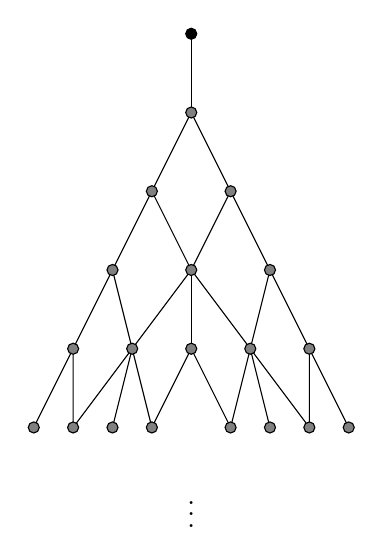
\begin{tikzpicture}[nodes={circle, draw, fill=black!50, inner sep=0pt, minimum width=4pt}]
              \draw (2,-4) -- (1.5,-3) -- (1,-2) -- (0.5,-1) -- (0,0) -- (-0.5,-1) -- (-1,-2) -- (-1.5,-3) -- (-2,-4);
        \draw (1.5,-3) -- (1.5,-4) -- (0.75,-3) -- (0,-2) -- (-0.75,-3) -- (-1.5,-4) -- (-1.5,-3);
        \draw  (1,-4) -- (0.75,-3) -- (0.5,-4) -- (0,-3) -- (-0.5,-4) -- (-0.75,-3) -- (-1,-4);
        \draw (0,-3) -- (0,-2);
        \draw (0.5,-1) -- (0,-2) -- (-0.5,-1);
        \draw (-0.75,-3) -- (-1,-2);
        \draw (0.75,-3) -- (1,-2);
        \draw (0,1) -- (0,0);
        \node[fill=black] at (0,1) {};
        \node at (0,0) {};
        \node at (-0.5,-1) {};
        \node at (0.5,-1) {};
        \node at (0,-2) {};
        \node at (1,-2) {};
        \node at (-1,-2) {};
        \node at (0,-3) {};
        \node at (0.75,-3) {};
        \node at (-0.75,-3) {};
        \node at (1.5,-3) {};
        \node at (-1.5,-3) {};
        \node at (-2,-4) {};
        \node at (-1.5,-4) {};
        \node at (-1,-4) {};
        \node at (-0.5,-4) {};
        \node at (0.5,-4) {};
        \node at (1,-4) {};
        \node at (1.5,-4) {};
        \node at (2,-4) {};
        \node[draw=none, fill=white] at (0,-5) {$\vdots$};
      \end{tikzpicture}
    \end{center}

with the root corresponding to the upper vertex of the square. 

\begin{prop}\label{grad}
Let $\mathfrak{t}$ be a bounded t-structure on $\mathscr{D}$, $\mathscr{P}$ an abelian $\mathbb{Z}$-slicing on $\heartsuit_{\mathfrak{t}}$, $\mathscr{Q}$ the associated $\mathbb{Z} \ltimes \hat{\mathbb{Z}}$-slicing on $\mathscr{D}$, $p$ a perversity. We have: 
\begin{enumerate}
\item if $\mathscr{P}$ is a perverse filtration, then $\mathscr{Q}$ satisfies the assumptions of \hyperref[pipp]{\textbf{Proposition \ref*{pipp}}} with respect to the map $\mathbb{Z} \ltimes \hat{\mathbb{Z}} \overset{f_p}{\longrightarrow} \mathbb{Z} \ltimes \hat{\mathbb{Z}}$ given by $$f_p(n,\phi)=(n+p(\lfloor \phi / 2 \rfloor),-p(\lfloor \phi / 2 \rfloor))$$ 
\item if $\mathscr{P}$ is a grading filtration, then $\mathscr{Q}$ satisfies the assumptions of \hyperref[pipp]{\textbf{Proposition \ref*{pipp}}} with respect to the map $\mathbb{Z} \ltimes \hat{\mathbb{Z}} \overset{g_p}{\longrightarrow} \mathbb{Z} \ltimes \hat{\mathbb{Z}}$ given by $$g_p(n,\phi)=(n+p(\phi),-p(\phi))$$ 
\item if $\mathscr{P}$ is a mixed filtration, then the abelian $\mathbb{Z}$-slicing induced on the heart of the bounded t-structure associated to $(g_p)_{\textnormal{\Libra}}(\mathscr{Q})$ is split 
\end{enumerate}
\end{prop}

\begin{proof}
Let's prove \textit{(2)}. Suppose $g_p(n,\phi) > g_p(m,\psi)$. Then either $m-n< p(\phi) - p(\psi)$ or both $m-n = p(\phi) - p(\psi)$ and $p(\psi) < p(\psi)$. Since by definition of t-structure we can assume $m \ge n$, the second case is absurd while in the first case, since $p$ is monotone, we have $\phi \ge \psi$ and thus by definition of perversity $$m-n<p(\phi)-p(\psi) \le \phi - \psi$$ 
and we get the desired Hom-vanishing by definition of grading filtration. \\

Suppose now $f_p(n,\phi) + 1 > f_p(m,\psi)$ and $(n+1,\phi) < (m,\psi)$. The only non absurd case is $ 1<m-n \le  p(\phi) - p(\psi)$. But then again we have $$2 \le m-n \le p(\phi)-p(\psi) \le \phi - \psi$$
and we can conclude as above. \\

To prove \textit{(1)} consider the monotone map $$\mathbb{Z} \overset{\lfloor * / 2 \rfloor}{\longrightarrow} \mathbb{Z}$$
Applying the slice functor to the latter and starting with a perverse filtration, we get a grading filtration by the properties of the floor function and the thesis follows from part \textit{(2)}. \\ 

Let's prove \textit{(3)}. We have to show that $$\mathscr{P}_{\psi}[1-p(\psi)] \subseteq \mathscr{P}_{\phi }[p(\phi)]^{\perp}$$ 
for $-p(\psi)>-p(\phi)$. We denote $n=p(\phi)-p(\psi)-1$. Assuming again $n \ge 0$, we have $n \ge 0 > p(\psi) - p(\phi) \ge \psi - \phi$ and we can then conclude by definition of mixed filtration. 
\end{proof}

Thus, in the presence of a grading (or perverse) filtration on the heart of a bounded t-structure, associating to a perversity $p$ the bounded t-structure coming from $(g_p)_{\textnormal{\Libra}}(\mathscr{Q})$ defines a morphism of $\mathbb{Z}$-posets $$\Xi^{\textnormal{op}} \longrightarrow \mathfrak{bts}(\mathscr{D})$$
we can restate this as: 

\begin{center}
\twonotes \ \textit{A grading or perverse filtration on the heart of a bounded t-structure on $\mathscr{D}$ induces a presheaf of t-structures on $\mathbb{Z} \times \mathbb{Z}$ with the product order, and thus some kind of a 'non totally ordered $\mathbb{Z} \times \mathbb{Z}$-slicing' on $\mathscr{D}$.}
\end{center}

\begin{center}
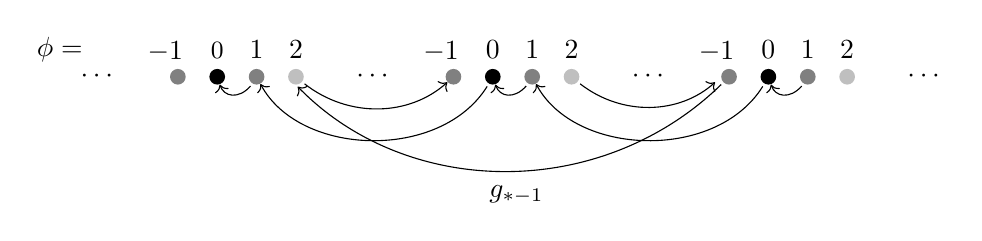
\begin{tikzpicture}

\node at (-5,0) {$\cdots$};
\draw (-4,0) node[circle,fill=gray,inner sep=2pt,label={[xshift=-4.5pt, yshift=-1pt]above: $-1$}] {};
\draw (-3.5,0) node[circle,fill,inner sep=2pt,label={[font=\small]above: $0$}] {};
\draw (-3,0) node[circle,fill=gray,inner sep=2pt,label=above: {$1$}] {} edge[->, bend left=60,looseness=1.5,shorten <=1pt,shorten >=3pt] (-3.5,0);
\draw (-2.5,0) node[circle,fill=lightgray,inner sep=2pt,label=above: {$2$}] {} edge[->, bend right=40,shorten <=1pt,shorten >=3pt] (-0.5,0);

\node at (-1.5,0) {$\cdots$};
\draw (-0.5,0) node[circle,fill=gray,inner sep=2pt,label={[xshift=-4.5pt, yshift=-1pt]above: $-1$}] {};
\draw (0,0) node[circle,fill,inner sep=2pt,label=above: {$0$}] {}  edge[->, bend left=60,shorten <=1pt,shorten >=3pt] (-3,0);
\draw (0.5,0) node[circle,fill=gray,inner sep=2pt,label=above: {$1$}] {} edge[->, bend left=60,looseness=1.5,shorten <=1pt,shorten >=3pt] (0,0);
\draw (1,0) node[circle,fill=lightgray,inner sep=2pt,label=above: {$2$}] {}  edge[->, bend right=40,shorten <=1pt,shorten >=3pt] (2.9,0);
\node at (2,0) {$\cdots$};

\draw (3,0) node[circle,fill=gray,inner sep=2pt,label={[xshift=-4.5pt, yshift=-1pt]above: $-1$}] {} edge[->, bend left=45,shorten <=1pt,shorten >=5pt] (-2.6,0);
\draw (3.5,0) node[circle,fill,inner sep=2pt,label=above: {$0$}] {} edge[->, bend left=60,shorten <=1pt,shorten >=3pt] (0.5,0);
\draw (4,0) node[circle,fill=gray,inner sep=2pt,label=above: {$1$}] {} edge[->, bend left=60,looseness=1.5,shorten <=1pt,shorten >=3pt] (3.5,0);
\draw (4.5,0) node[circle,fill=lightgray,inner sep=2pt,label=above: {$2$}] {};
\node at (5.5,0) {$\cdots$};

\node at (-5.5,0.35) {$\phi=$};
\node at (0.3,-1.5) {$g_{*-1}$};

\end{tikzpicture}
\end{center}

Now, by sending an upper set of $I \in O(\mathbb{Z})$ to its characteristic function $\chi_I$ we get an embedding $$O(\mathbb{Z})^{\textnormal{op}} \hookrightarrow \Xi$$ and the t-structure coming from $(g_{\chi_I})_{\textnormal{\Libra}}(\mathscr{Q})$ is just the tilting of $\mathfrak{t}$ with respect to the torsion pair coming from $I$. \\
The following proposition gives a characterization of the new heart obtained by the above construction. In the case of a mixed filtration, we get a splitting property which is often referred as 'decomposition theorem for perverse sheaves' in literature. \\

\begin{prop}
Let $\mathfrak{t}$ be a bounded t-structure on $\mathscr{D}$, $\mathscr{P}$ a grading filtration on $\heartsuit_{\mathfrak{t}}$, $\mathscr{Q}$ the associated $\mathbb{Z} \ltimes \hat{\mathbb{Z}}$-slicing on $\mathscr{D}$, $p$ a perversity. Denote $\mathfrak{q}$ the bounded t-structure associated to $(g_p)_{\textnormal{\Libra}}(\mathscr{Q})$. Then $\heartsuit_{\mathfrak{q}}$ consists of objects $X \in \mathscr{D}$ so that $$H_{\mathfrak{t}}^{k}(X) \in \mathscr{P}_{p^{-1}(-k)}[k]$$ 
for each $k \in \mathbb{Z}$. Moreover, if $\mathscr{P}$ is a mixed filtration then for each $X \in \heartsuit_{\mathfrak{q}}$ $$X=\bigoplus_{n \in \mathbb{Z}}H_{\mathfrak{t}}^{n}(X)$$ 
\end{prop}

\begin{proof}
This is very similar to \hyperref[tilt1]{\textbf{Proposition \ref*{tilt1}}}: we have that $X \in \heartsuit_{\mathfrak{q}}$ if and only if $$H_{\mathscr{P}}^{\phi}(H_{\mathfrak{t}}^k(X)[-k])[k]=H_{\mathscr{Q}}^{(k,\phi)}(X)=0$$ 
for $p(\phi) \not = -k$. \\
For the second part of the claim, the abelian $\mathbb{Z}$-slicing induced on $\heartsuit_{\mathfrak{q}}$ is split by \hyperref[grad]{\textbf{Proposition \ref*{grad}}} and thus by \hyperref[split]{\textbf{Proposition \ref*{split}}} $$X=\bigoplus_{(k,\phi)}H_{\mathscr{Q}}^{(k,\phi)}(X)=\bigoplus_{n \in \mathbb{Z}}H_{\mathfrak{t}}^{n}(X)$$
where the last equality comes from the first part. 
\end{proof}

\begin{exmp}
Let $$B=\bigoplus_{i\in \mathbb{N}}B_i$$ be an $\mathbb{N}$-graded ring with $B_0$ semisimple. Denote $\mathscr{A}$ the category of $\mathbb{Z}$-graded $B$-modules with only finitely many nonzero graded pieces. For $\phi \in \mathbb{Z}$, denote $\mathscr{P}_{\phi}$ the full subcategory of $\mathscr{A}$ of modules concentrated in degree $\phi$. Clearly, $\mathscr{P}$ defines an abelian $\mathbb{Z}$-slicing on $\mathscr{A}$. Following \cite{kos} we have $$\textnormal{Ext}_{\mathscr{A}}^n(\mathscr{P}_{\phi},\mathscr{P}_{\psi})=0$$
for $n>\psi - \phi$. This means that $\mathscr{P}$ is a mixed filtration and the bounded t-structure on $\mathscr{D}^b(\mathscr{A})$ associated to $(g_1)_{\textnormal{\Libra}}(\mathscr{Q})$ (where $1$ is the identity of $\mathbb{Z}$) is the 'diagonal' (or 'geometric') t-structure which appears in Koszul duality and other areas. 
\end{exmp}

\begin{exmp}
Let $M$ be an $n$-dimensional smooth complex projective variety and consider the $n$-torsion pair $\mathscr{P}$ on $\textnormal{Coh}(M)$ from \hyperref[cohh]{\textbf{Example \ref*{cohh}}}. Using Serre duality and the Grothendieck vanishing theorem, one sees that $\mathscr{P}$, seen as an abelian $\mathbb{Z}$-slicing via the inclusion $[n] \subseteq \mathbb{Z}$, is a perverse filtration. The bounded t-structure associated to $(f_p)_{\textnormal{\Libra}}(\mathscr{Q})$ is the one of perverse coherent sheaves as constructed in \cite{bez}. Following again the proof of \hyperref[t]{\textbf{Proposition \ref*{t}}}, we can use the Harder-Narasimhan filtrations from Gieseker stability to obtain an abelian $J_n$-slicing on the heart of perverse coherent sheaves as done in \cite{perpol}. 
\end{exmp}

Now we somehow review the gluing construction for t-structures in \cite{del}, but generalize it to any slicing. Our language is quite different though, and we formulate the problem very similarly to \cite{glu}. We start with two $\mathbb{Z}$-posets $J,J'$. 

\begin{defn}
Let $\mathscr{P}$ be a $J \ltimes J'$-slicing on $\mathscr{D}$. We call $\mathscr{P}$ \textbf{gluable} if it satisties the assumptions of \hyperref[pipp]{\textbf{Proposition \ref*{pipp}}} with respect to the map $J \ltimes J' \overset{e}{\longrightarrow} J' \ltimes J$ that exchanges coordinates. In this case we denote $$\overline{\mathscr{P}}=e_{\textnormal{\Libra}}(\mathscr{P})$$
\end{defn}

By a simple computation, the gluability condition reads: $\mathscr{P}_{(\phi,\psi)} \subseteq \mathscr{P}_{(\phi',\psi')}^{\perp}$ if $\psi' > \psi$ or both $\psi'+1>\psi$ and $\phi'+1 < \phi$. For example, the first condition is automatic when $\mathbb{Z}$ acts trivially on $J$ (in this case, it follows from the second one). In particular, if $\mathbb{Z}$ acts trivially on $J$, $\mathscr{P}$ is a $J$-slicing on $\mathscr{D}$ and $\mathfrak{t}_{\phi}$ is a bounded t-structure on $\mathscr{P}_{\phi}$ for each $\phi \in J$, then using \hyperref[aab]{\textbf{Proposition \ref*{aab}}} we get a $J \ltimes \mathbb{Z}$-slicing $\mathscr{Q}$ which is gluable if and only if $$\heartsuit_{\mathfrak{t}_{\psi}}[n] \subseteq \heartsuit_{\mathfrak{t}_{\phi}}^{\perp}$$
whenever both $n \le 0$ and $\phi < \psi$. 

\begin{rem}
We have a commutative diagram of $\mathbb{Z}$-posets 
\begin{center}
\begin{tikzcd}[ampersand replacement=\&]
\mathbb{Z} \ltimes \mathbb{Z} \arrow{r}{\sim} \arrow{d}{e} \& \mathbb{Z} \ltimes \hat{\mathbb{Z}} \arrow{d}{g} \\
\mathbb{Z} \ltimes \mathbb{Z} \arrow{r}{\sim}  \& \mathbb{Z} \ltimes \hat{\mathbb{Z}} 
\end{tikzcd}
\end{center}
where the horizontal isomorphism is the one from \hyperref[zet]{\textbf{Remark \ref*{zet}}}. Indeed, a $\mathbb{Z} \ltimes \mathbb{Z}$-slicing on $\mathscr{D}$ is gluable if and only if it induces a grading filtration on the heart of the associated t-structure when seen as a $\mathbb{Z} \ltimes \hat{\mathbb{Z}}$-slicing. 
\end{rem} 

An easy combinatorial calculation finally yelds the following two remarks: 
\begin{itemize}
\item  if $\mathscr{P}$ is a gluable $\hat{\mathbb{Z}} \ltimes \mathbb{Z}$-slicing on $\mathscr{D}$, then $\overline{\mathscr{P}}$ induces a grading filtration on the associated heart, allowing us again to construct new bounded t-structures depending on a perversity. 
\item if $\mathscr{P}$ is a mixed filtration on the heart of a bounded t-structure and $\mathscr{Q}$ is the associated $\mathbb{Z} \ltimes \hat{\mathbb{Z}}$-slicing on $\mathscr{D}$, then $\mathscr{Q}$ is gluable. In this case, looking at $\overline{\mathscr{Q}}$, we get a baric structure on $\mathscr{D}$ which is usually called \textbf{weight decomposition} in literature. 
\end{itemize}
In other words, the chain of implications for a $\mathbb{Z} \ltimes \hat{\mathbb{Z}}$-slicing refines to 
$$\textnormal{mixed} \implies \textnormal{gluable} \implies \textnormal{grading} \implies \textnormal{perverse} $$

%\begin{prop}
%A $J \ltimes J'$-slicing $\mathscr{P}$ on $\mathscr{D}$ is gluable if and only if it satifies the assumptions of \hyperref[pipp]{\textbf{Proposition \ref*{pipp}}} with respect to the identity (as sets) $J \ltimes J' \longrightarrow J \times J'$, where we place the product order on the right member. 
%\end{prop}
%
%\begin{proof}
 % Consider the following commutative diagram of sets
 % \begin{center}
%\begin{tikzcd}[ampersand replacement=\&]
%J \ltimes J' \arrow{r}{e} \arrow{d}{1} \& J \ltimes J' \\
%J \times J' \arrow{r}{e}  \& J \times J' \arrow{u}{1}
%\end{tikzcd}
%  \end{center}
%  The right arrow is a morphism of $\mathbb{Z}$-posets while the down one is an isomorphism of $\mathbb{Z}$-posets, and the thesis follows. 
%\end{proof}
%\begin{prop}
%Let $\mathscr{P}$ be a gluable $J \times J'$-slicing on $\mathscr{D}$. For $i = 1,2$, denote $\mathscr{P}^i=\pi_{\textnormal{\Libra}}^i(\mathscr{P})$, where $J \overset{\pi^1}{\longleftarrow} J \times J' \overset{\pi^2}{\longrightarrow} J'$ are the projections. Then for each $\psi \in J'$, $\mathscr{P}_{\psi}^2$ consists of objects $X \in \mathscr{D}$ so that $$H_{\mathscr{P}^1}^{\phi}(X) \in \mathscr{Q}_{(\phi,\psi)}$$
%for each $\phi \in J$.
%\end{prop}
%
%\begin{proof}
%We have already seen that $X \in \mathscr{P}_{\psi}^2$ if and only if $$H_{\mathscr{P}}^{\lambda}(X)=H_{\mathscr{P}}^{\lambda}(H_{\mathscr{P}^1}^{\pi^1(\lambda)}(X))=0$$
%for $\pi^2(\lambda) \not =\psi$. By fixing $\pi^1(\lambda)=\phi$ and varying $\pi^2(\lambda)$, we get the desired result. 
%\end{proof}
\newpage



\afterpage{\blankpage}
\clearpage 
\bibliographystyle{alpha}

\end{document}
